\documentclass{article}
\usepackage[utf8]{inputenc}
\usepackage{physics}
\usepackage{enumitem}
\usepackage{graphicx}
\usepackage{subcaption}
\usepackage{float}
\usepackage{amsmath}
\usepackage{amssymb}
\usepackage{setspace}
\usepackage{xfrac}
\usepackage{indentfirst}
\usepackage{tikz}
\usepackage{hyperref}
\usepackage{tikz}
\usetikzlibrary{positioning, fit, calc, arrows,shapes.gates.logic.US,shapes.gates.logic.IEC,}
\usepackage[siunitx, RPvoltages]{circuitikz}

\title{ECE210 Final Review - Cramming Carnival}
\author{Author: Members of HKN}
\date{Fall 2024}


\usepackage[makeroom]{cancel}
\usepackage[letterpaper, portrait, margin=1in]{geometry}
\usepackage{graphicx}

\pagenumbering{arabic}

\begin{document}

\maketitle

Note: Problems with three stars are more difficult than what you'd see on a final exam. They will teach you a lot if you do them, but don't be worried if you get stuck on them. Everything else is either at exam-level or easier.

\section{Fabled Fourier}

Determine the Fourier transform of the following:
\begin{enumerate}
    \item $f(t) = \text{sinc}(4t-8) * -\text{rect}(t)$
    \item $g(t) = \frac{1}{(4 + jt)^2}$
    \item $h(t) = \text{sinc}^2(3t-3)$
    \item $h'(t)$, using $h(t)$ defined above
\end{enumerate}
\vfill
\section{Scintillating Simplfications}

Simplify the following expressions:

a. $f(t) = (t^2 + 1)\delta(t - 1)\delta(t + 1)$

b. $g(t) = (t^2 + 1)(\delta(t - 1) + \delta(t + 1))$

c. $h(t) = (t^2 + 1) * (\delta(t - 1) + \delta(t + 1))$

\vfill
\newpage

\section{Clever Components}The component represented as a box in the following problem has the following time-domain I-V relationship.

\[
V(t) = K\dv[2]{I(t)}{t}
\]

Let $v(t) = \sin(t)$, and let $K_1 = 4$. Assume all initial conditions are 0 in the circuit, aside from the driving force $v(t)$. Given the circuit below, answer the following questions.

\begin{figure}[ht!]
\centering
\begin{circuitikz}[american, transform shape, voltage dir = old]
\draw (-1,0) to[R, l_=$K_1$, european] ++ (0,-3) to[short] ++ (-3,0)
		to[V=$v(t)$] ++ (0,3) to[R, l^=$2\,\unit{\ohm}$] ++ (3,0);

\draw (-0.7,0) to[open, v=$ $] ++ (0,-3);
\node at (-0.7,-1.5) [anchor=west]{$v_x(t)$};
\end{circuitikz}
\end{figure}

\paragraph{a)} What are the units of $K$? Use at most two other units in your answer.

\paragraph{b)} Find the voltage $v_x(t)$, in the time domain, using only real functions.

\vfill

\section{Illuminating Impulse Response}

Consider an LTI system where the input $f(t) = 5u(t)$ results in a zero-state response $y(t) = e^{5t}u(t)$. Find the impulse response of the system. Also state if the system is causal and/or BIBO-stable. If it isn't BIBO-stable, name a bounded input that will cause an unbounded output.

\vfill
\newpage


\section{Tremendous Transformations}

Determine the Thevenin equivalent of the following network between nodes $a$ and $b$, and then determine the available power of the network:

\begin{figure}[h]
\begin{center}
    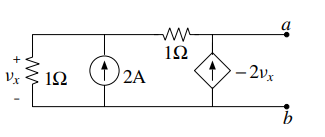
\includegraphics[width=0.5 
    \textwidth]{figures/qqqq.PNG}
\end{center}
\end{figure}

\vfill

\section{Legendary Laplace}

\begin{itemize}
    \item Find the Laplace Transform of $x(t) = e^t u(-t)$.
    \item Find the Laplace Transform of $x(t) = rect(t - \frac{1}{2})$.
\end{itemize}

\vfill

\section{Iconic Inverses}

\begin{itemize}
    \item Find the inverse Laplace Transform of $\hat{H}(s) = \frac{1}{s(s^2 + 2s + 2)}$.
    \item Find the inverse Laplace Transform of $\hat{H}(s) = e^{-4s}\frac{6s-1}{(s+1)^2(s-2)}$.
\end{itemize}

\vfill

\newpage
\section{Perplexing Poles}

Determine the poles and ROC of the following transfer function, and determine if it represents a BIBO-stable LTIC system.

$$\hat{H}(s) = \frac{s^4(s + 3)}{(s^2 + 5s + 6)}$$

\vspace{4cm}

\section{Exquisite Electronics}

Let $f(t)$ be the input to the following circuit, with $y(t)$ denoted as:

\begin{figure}[h]
\begin{center}
    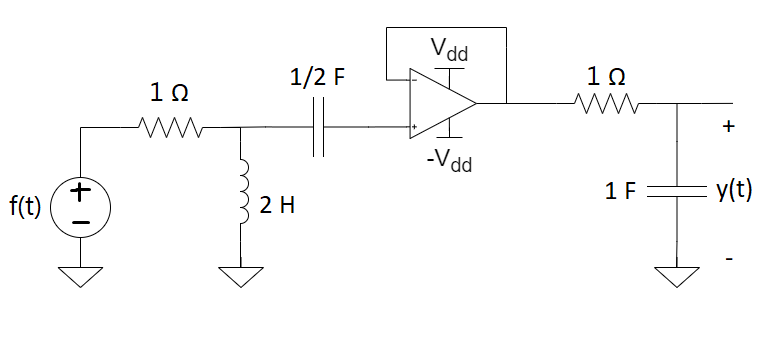
\includegraphics[width=0.5 
    \textwidth]{figures/circuit7.png}
\end{center}
\end{figure}

Find the circuit's transfer function in the time domain.
\newpage

\section{Delightful Differential}

Consider an LTIC system described by the ODE

$$\frac{d^2y}{dt^2}+\frac{dy}{dt}-2y(t) = f(t)$$

with initial conditions $y(0^-) = 3$ and $y'(0^-) = 8$.

Determine the system's transfer function $\hat{H}(s)$, its characteristic polynomial, characteristic poles, characteristic modes, and zero-input solutions in both the $s$ domain and the time domain. Also note if the system is BIBO stable or not and say why.

\vfill

\section{Insidious Inputs}

Let a system be defined by its input-output relation $y(t) = x(102841) + x(t)$. Is the system Linear? Time-Invariant? BIBO-Stable? Causal? If it is BIBO-Unstable, name a bounded input that will cause an unbounded output.

\vfill

\section{Outrageous Outputs}

Let a system be defined by the following input-output relation:
$$y(t) =
    \begin{cases}
      9^t x(t-4) & , -\infty < t \leq 10^6\\
      sin^3(t+4) cos(t+2) x(t-1) & , 10^6 < t < \infty
    \end{cases}$$    
Is the system Linear? Time-Invariant? BIBO-Stable? Causal? If it is BIBO-Unstable provide a bounded input that causes an unbounded input.

\vfill

\newpage

%\section{Calculated Convolution}

%Determine and sketch $y(t) = f(t) * h(t)$ where $f(t) = e^{-2t}u(t)$ and $h(t) = rect(\frac{t}{4})$.

\section{Unpopular Unit-step}

Let a system be defined by its impulse response $h(t) = u(t)$. Is the system Linear? Time-Invariant? Causal? BIBO-Stable? If it is BIBO-Unstable, name a bounded input that will cause an unbounded output.

\vspace{3cm}

\section{Disgusting Derivative}

Let a system be defined by the input-output relation $y(t) = \frac{dx}{dt}$. Is the system Linear? Time-Invariant? BIBO-Stable? Causal? If it is BIBO-Unstable provide a bounded input that causes an unbounded input.
\vfill

\section{Peculiar Plots}

Let $f(t) = 7e^{j5t} sinc^2(\frac{5t}{2})$ be the input into a system with the following impulse response:

%\begin{figure}[h]
%\begin{center}
%    \includegraphics[width=
%    \textwidth]{figures/System Response.jpg}
%\end{center}
%\end{figure}

\begin{figure}[h!]
    \centering
    \begin{tikzpicture}
    %Magnitude Plot
    \draw[<->, thick] (-7,-1)--(-1,-1) node[anchor=east, above=2pt]{$\omega$};
    \draw[<->, thick] (-4,-1.5) -- (-4,1.5) node[anchor=south, left=2pt]{$|H(\omega)|$};
    %magnitude line
    \draw[<->] (-7,0.5) -- (-3.75,0.5)node[anchor=mid, above ]{2} -- (-1,0.5) ;

    %Phase Plot
    \draw[<->, thick] (1,0) -- (7,0) node[anchor=east, above=2pt]{$\omega$};
    \draw[<->, thick] (4,-2) -- (4,2) node[anchor=south, left=2pt]{$\angle H(\omega)$};
    %phase line
    \draw[<->] (2,-2) -- (6,2);
    \draw (3.9,1) node[anchor = east]{$\pi$} -- (4.1,1);
    \draw (5,-0.1) node[anchor = north]{1} -- (5,0.1);
    \draw[dashed, thin] (4,1) -- (5,1) -- (5,0);
    
    \end{tikzpicture}
\end{figure}

What is the output?

\vfill

\newpage

\section{Cataclysmic Convolution}

Given:$$f(t) = \frac{\cos(t)}{t},\, g(t) = \frac{\sin(t)}{t^2}, h(t) = \text{rect}\bigg(\frac{t}{2}\bigg)$$

Find $\big(f(t)*h(t)\big) - \big(h(t)*g(t)\big)$. $\textbf{Hint:}$ there's a derivative somewhere...

\vfill

\section{Rambunctious Reality}

Given the Fourier transform $F(\omega) = \omega^2cos(2\omega)sin^2(\pi\omega) + j2sin(\tau\omega)$, prove that the corresponding $f(t)$ is a real signal. You don't need to solve for $f(t)$.

\vfill

\newpage


\section{Perceptive Proofs}

\subsection{Meritorious Modulation}
Without using the modulation property, show that $f(t)\cos(\omega_c t)$ transforms to $\frac{1}{2}\big[F(\omega - \omega_c) + F(\omega + \omega_c)\big]$.
\vfill

\subsection{Immutable Invariance***}
Prove an impulse train transforms into another impulse train, without explicitly using transforms 24 or 25 in your tables. 
\newline
$\textbf{Bonus:}$ What condition must be true for the impulse train's period to be invariant under the Fourier Transform?
Recall that the impulse train has the following form, where $T$ is the period:

$$\sum_{n = -\infty}^{\infty} \delta(t - nT)$$

\vfill


\subsection{Fantastic Four}
Prove that applying the Fourier transform four times to a function returns the original function, scaled by some positive scaling factor $K > 1$. Also, find $K$.

\vfill

\newpage


\section{Fatal Feedback***}

Find the transfer function of the following circuit in the s-domain.

\begin{figure}[ht!]
\centering
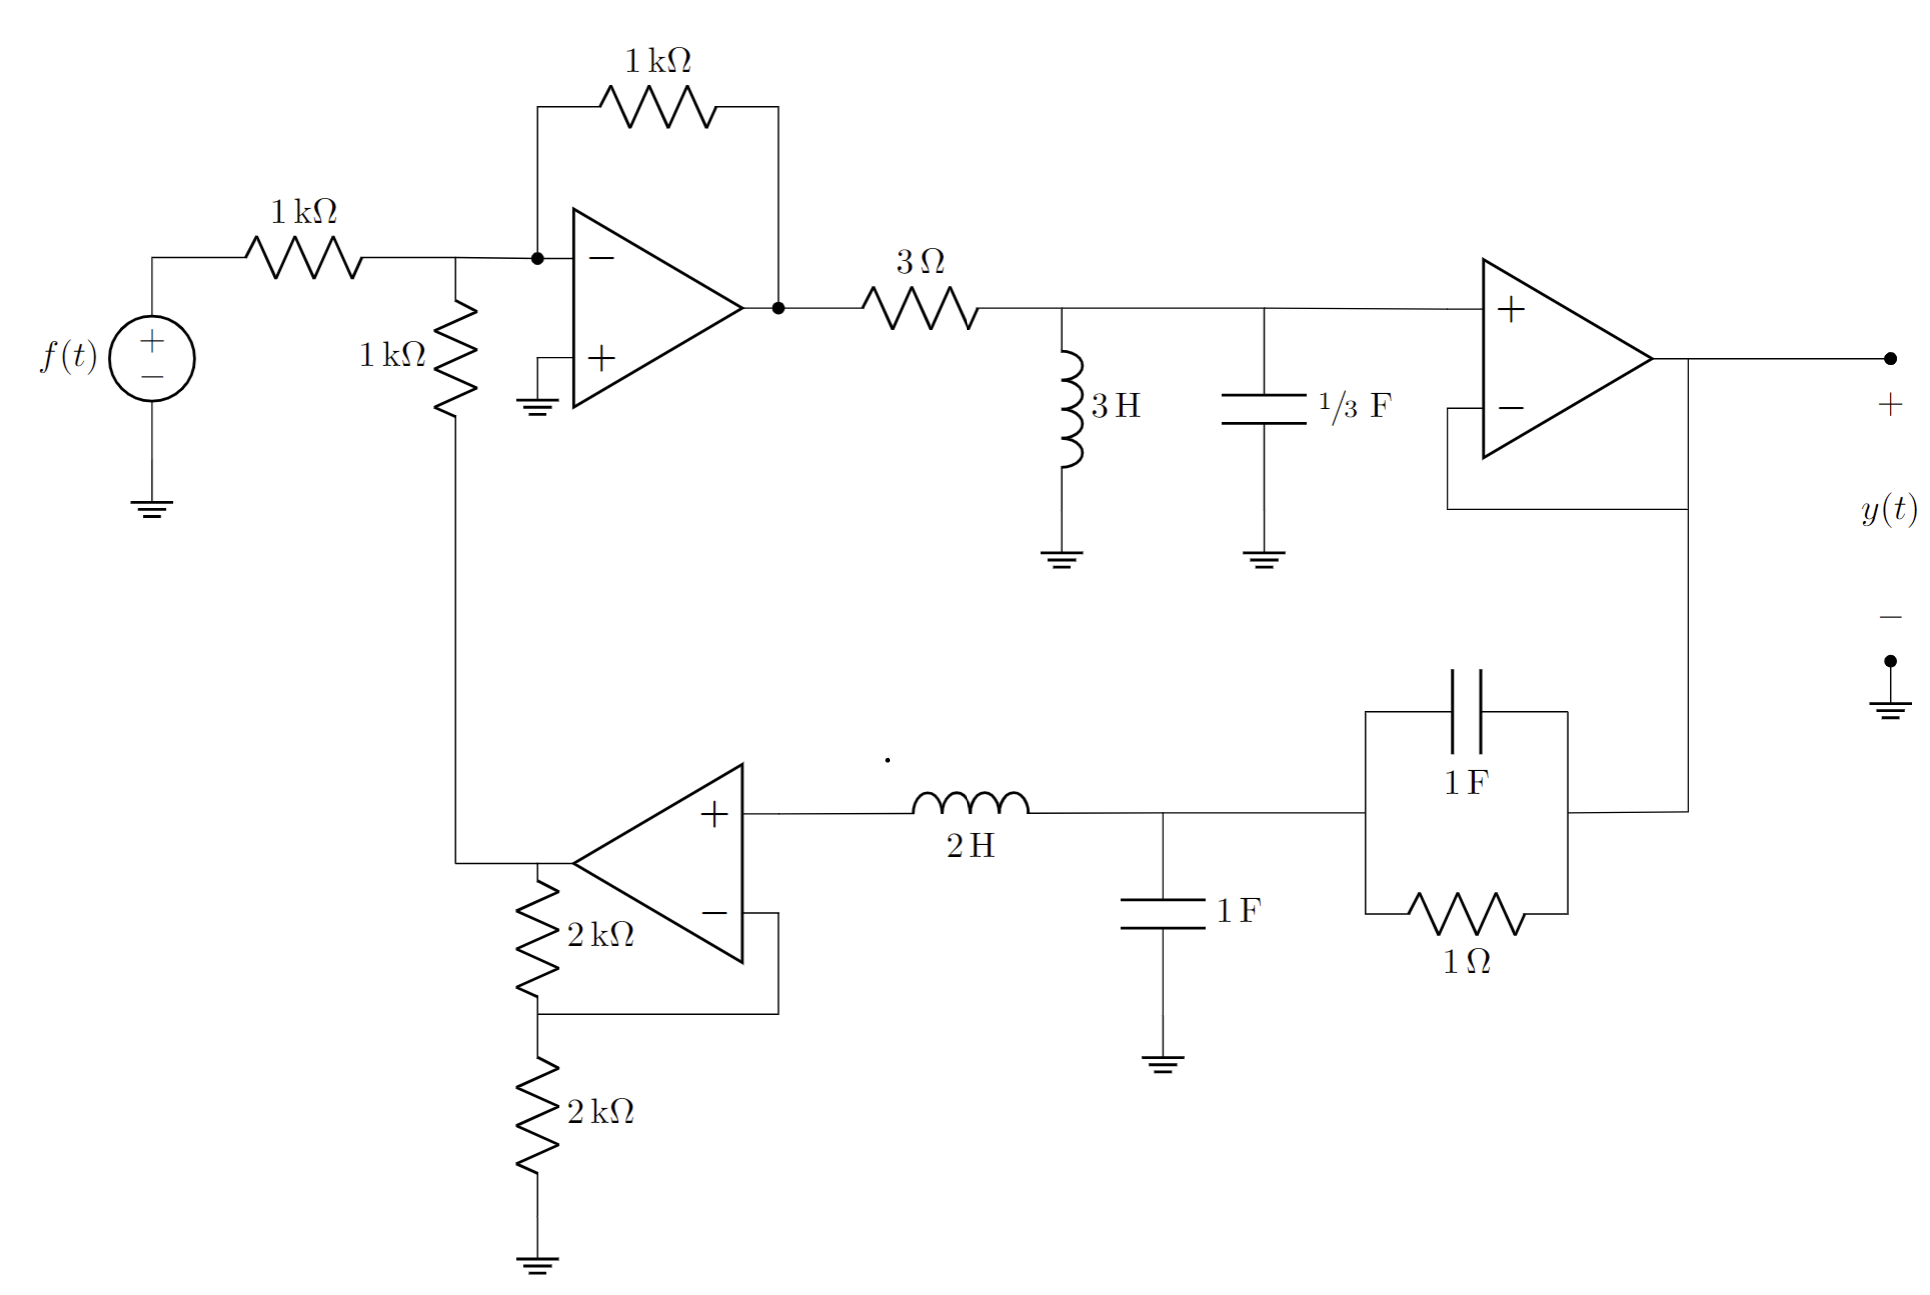
\includegraphics[width=0.8\linewidth]{figures/mega.png}
\end{figure}

\newpage


\end{document}